\documentclass{article}

\usepackage{graphicx}
\usepackage{tikz}
\usepackage{tikzsymbols}
\usetikzlibrary{calc,patterns,shapes.geometric}
\pagestyle{empty}
\usepackage[margin=0pt]{geometry}
\geometry{papersize={14in,12in}}

\def\centerarc[#1](#2)(#3:#4:#5){\draw[#1] ($(#2)+({#5*cos(#3)},{#5*sin(#3)})$) arc (#3:#4:#5);}

\begin{document}
	\begin{figure}
		\centering
		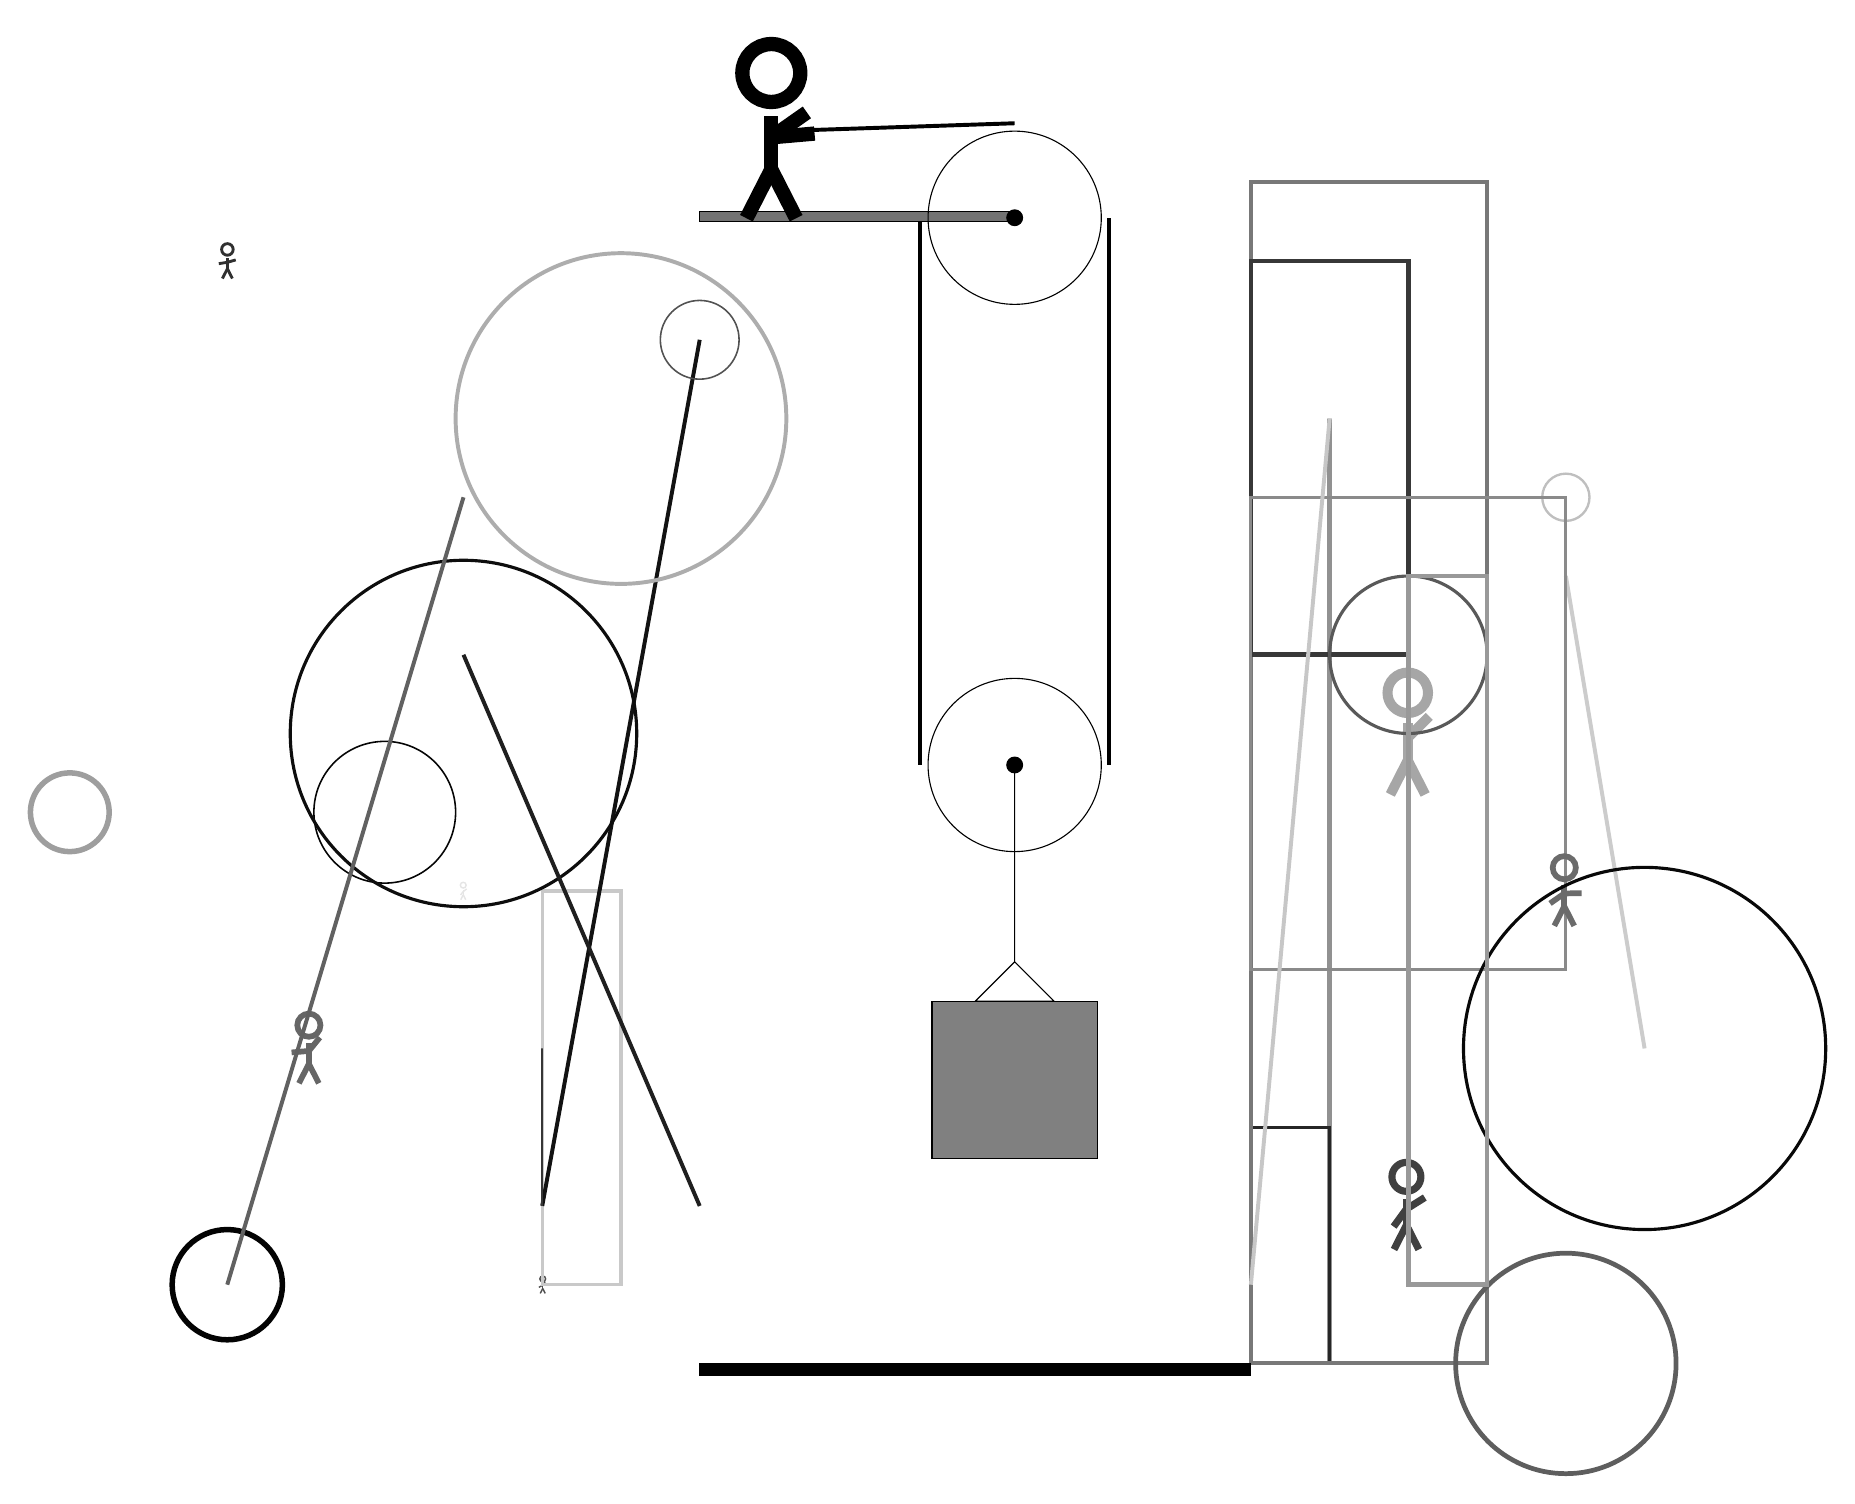
\begin{tikzpicture}
			%%%%% START %%%%%
			
			\draw[fill=black!55] (-2, 11.5) rectangle (2, 11.625);
			
			\draw (2, 4.6) circle (1.1);
			\draw[fill=black] (2, 4.6) circle (0.1);
			
			\draw (2, 11.55) circle (1.1);
			\draw[fill=black] (2, 11.55) circle (0.1);
			
			\draw (2, 4.6) -- (2, 2.1) -- (1.5, 1.6) -- (2.5, 1.6) -- (2, 2.1);
			\draw[fill=black!50] (0.95, 1.6) rectangle (3.05, -0.4);
			
			\draw[line width=0.5mm] (0.8, 11.5) -- (0.8, 4.6);
			\centerarc[line width=0.5mm](2, 4.6)(180:360:1.2000000000000002);
			\draw[line width=0.5mm](3.2, 4.6) -- (3.2, 11.55);
			\centerarc[line width=0.5mm](2, 11.55)(0:90:1.2000000000000002);
			\draw[line width=0.5mm](2, 12.75) -- (-1, 12.65);
			
			\draw [line width=0.7mm, color=black!99](-8, -2) circle (0.7);
			
			\draw [line width=0.2mm, color=black!98](-6, 4) circle (0.9);
			\draw[line width=0.6mm, color=black!43] (6, -3) rectangle (6, 9);
			\node[line width=0.3mm, color=black!60] at (-7, 1) {\Strichmaxerl[4][5][51]};
			\draw[line width=0.5mm, color=black!20](9, 7) -- (10, 1);
			\node[line width=0.7mm, color=black!69] at (-4, -2) {\Strichmaxerl[1][27][56]};
			\draw[line width=0.4mm, color=black!85] (5, -3) rectangle (6, 0);
			\draw[line width=0.4mm, color=black!21] (-3, -2) rectangle (-4, 3);
			\draw[line width=0.5mm, color=black!53] (5, 12) rectangle (8, -3);
			\node[line width=0.4mm, color=black!35] at (7, 5) {\Strichmaxerl[7][90][45]};
			\node[line width=0.4mm, color=black!10] at (-5, 3) {\Strichmaxerl[1][52][38]};
			\draw [line width=0.7mm, color=black!38](-10, 4) circle (0.5);
			\node[line width=0.6mm, color=black!75] at (7, -1) {\Strichmaxerl[5][54][32]};
			
			\draw[line width=0.5mm, color=black!93](-4, -1) -- (-2, 10);
			\draw [line width=0.4mm, color=black!95](-5, 5) circle (2.2);
			\draw [line width=0.3mm, color=black!25](9, 8) circle (0.3);
			
			\draw[line width=0.6mm, color=black!78] (7, 6) rectangle (5, 11);
			\node[line width=0.4mm, color=black!81] at (-8, 11) {\Strichmaxerl[2][9][16]};
			\draw[line width=0.4mm, color=black!46] (5, 8) rectangle (9, 2);
			\draw [line width=0.4mm, color=black!65](7, 6) circle (1.0);
			\draw [line width=0.2mm, color=black!68](-2, 10) circle (0.5);
			\draw[line width=0.5mm, color=black!62](-5, 8) -- (-8, -2);
			\draw[line width=0.2mm, color=black!79] (-4, -1) rectangle (-4, 1);
			\draw [line width=0.6mm, color=black!63](9, -3) circle (1.4);
			\draw[line width=0.5mm, color=black!88](-2, -1) -- (-5, 6);
			\draw[line width=0.5mm, color=black!22](6, 9) -- (5, -2);
			\node[line width=0.3mm, color=black!58] at (9, 3) {\Strichmaxerl[4][35][1]};
			\draw [line width=0.4mm, color=black!97](10, 1) circle (2.3);
			\draw[line width=0.6mm, color=black!40] (7, -2) rectangle (8, 7);
			
			\draw [line width=0.5mm, color=black!32](-3, 9) circle (2.1);
			
			\node at (-1, 12.65) {\Strichmaxerl[10][-175][35]};
			
			\draw[fill=black] (-2, -3) rectangle (5, -3.15);
			
			%%%%% END %%%%%
		\end{tikzpicture}
	\end{figure}	
\end{document}